 \section{Functional Overview}
The functional overview of the AZ-SMART system is depicted in Figure \ref{figWorkflow}, showing multiple activities connected in a
sequential but also bi-directional workflow.  One can begin with the top-right of the diagram and work counter-clockwise to
understand the intended workflow pattern.  An AZ-SMART user will begin with the GIS tasks of compiling a database in the Geodatabase
that will contain all the needed information for the AZ-SMART system, with the exception of the travel model and a mid-level model
that will be interfaced to AZ-SMART (in a later phase, the mid-level model is likely to become a component of AZ-SMART rather than
an external process).

As the database is assembled in the gepdatabase, including all land use layers, environmental, planning and political boundaries,
development projects, and other related inputs, the AZ-SMART user will employ a suite of diagnostic tests to examine the database
for missing, erroneous, and inconsistent data, and will use editing and validation tools to repair problems, and impute values for
missing and erroneous data.  During this process, there would be considerable iteration between the data assembly step and the data
diagnostic step, as some input data might be replaced or updated.  This step would also involve the assembly of metadata concerning
the data sources, vintage, and any information developed on data quality.

The next step in the workflow is the development of models that are consistent with the database and can be used to allocate land
uses to small areas (we discuss the form of the data in detail in the data subsection).  The models used by AZ-SMART will be configured
to undertake land use allocation as described in the model subsection, and will be flexible with respect to the variables and weights
(parameters) used.  The models themselves will be modular and flexible to allow ongoing refinement over time by AZ-SMART users as they
gain insights into alternative means of doing the allocations.  This step also involves selecting the variables to use in each model
component, and estimating model parameters statistically, or if desired, inputting parameters manually for some model components.
The tools for model estimation will be internal to the system, allowing ease of re-estimation if the user wishes to experiment with
alternative specifications.  Diagnostics from model estimation, such as sensitivity to variables and correlation among variables,
will be available to assess the robustness and sensitivity of each model component.  The user will also be able to compare observed
to predicted data over an observed period if such data is available.  This model specification and calibration process may identify
problems in the data, which will require moving back upstream in the workflow process to refine input data.

Once the models are estimated and the system calibrated to the users' satisfaction, the model system may be put into use. Putting
the model into use requires the specification of one or more 'scenarios' that contain the input data that define the input conditions
and assumptions for a run of the model system, including control totals, land development constraints, development projects, and
transportation system.  These scenarios may involve graphical editing in the GIS environment, to edit boundaries of designated areas
or to generate buffers or distances from specified features such as access points on the transportation system.  The scenario
specification will also include controls for the interfacing of the travel model system (which years to run, what variables to pass,
for example), and the mid-level land use model system or the control totals that have been generated by them.

The next step in the workflow is to run one or more scenarios over a forecast period defined by the scenarios.  This may be done in
a batch mode that automates the entire modeling process from the loading of initial data for the base year, through multiple time
steps and exchanges with the travel model, and possibly the mid-level model, until completion of the entire modeling period of 30
or more years (for example).  In other cases, the user may wish to run a scenario only for a portion of the intended forecast period,
then stop the simulation to examine results, and possibly to make changes in the scenario assumptions that will shape the simulation
in the next section of the forecast period.  Yet another possibility is that the user will see patterns in the results that are not
desired, and decide to back up to the scenario specification stage, or even to the model specification stage, to make refinements
and resume the process.

Typically the process of examining simulation results will involve creating indicators and extracts (or summaries) of the detailed
simulation results.  We shall refer broadly to these as indicators.  The indicators may be simple aggregation of results, such as
housing units or acres of each land use sector by zone, or RAZ.  Or they may involve computations that are more complex, such as
estimating the remaining development capacity within each city.  The indicators may be produced as maps, or charts, or tables.
They may be of three types: snapshots (looking at an indicator for a single scenario and year), changes (usually from the base year
to some forecast year), and differences (usually between a specific scenario and a baseline scenario for a selected year).  It is
likely that many of these would be map indicators and be viewed in the GIS environment.


\clearpage

Simulation results may also be stored to the Geodatabase.  A user may wish to store either the full set of simulation results with
all of the intermediate calculations needed to understand or even re-start a simulation from an intermediate year, or alternatively
only a subset of specified results can be written to the Geodatabase for archiving and further visual examination.  The system will
provide tools for both use cases.

This brings the workflow full circle to the top-right, where the data used as inputs and the data produced by the simulation may all
be visually examined and edited.  Refinement of forecast results would be done at this stage also.  There are of course many possible
variants on this workflow description, and theoretically one could draw connections among almost any pair of these task components,
and the AZ-SMART system will support this kind of flexibility (but the diagram would be quite hard to interpret at that point).  The
next section moves to the system architecture perspective.

\begin{figure}[h]
\begin{center}
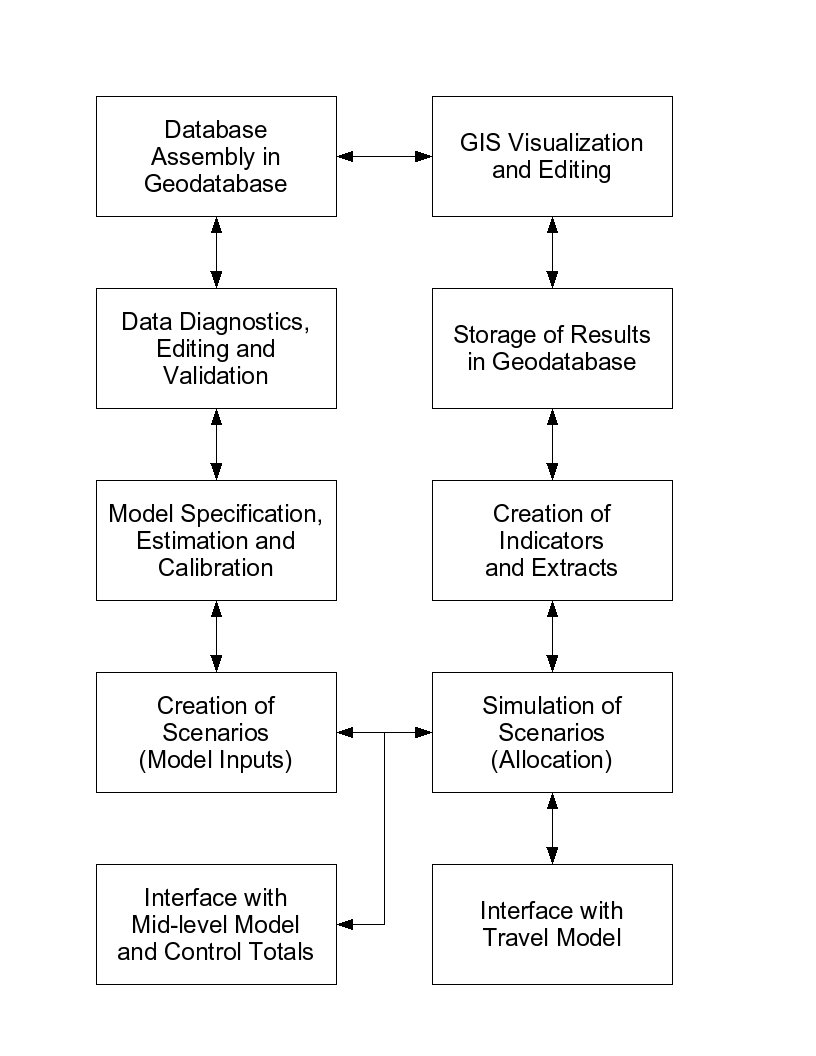
\includegraphics[scale=0.6]{figures/functional_diagram.png}
\caption{AZ-SMART Workflow Diagram}
\label{figWorkflow}
\end{center}
\end{figure}
